\documentclass{../c-lecture}

\subtitle{Arrays}

\begin{document}

\begin{frame}
  \titlepage{}
\end{frame}
\begin{frame}
  \frametitle{Outline}
  \tableofcontents{}
\end{frame}

\section{Introduction}

\begin{frame}
  \frametitle{Introduction}
  \begin{itemize}
    \item Algorithms usually work on large data sets
    \begin{itemize}
      \item Sort a set of numbers
      \item Search a specific number in a set of numbers
    \end{itemize}
    \item How to read and store a set of data?
    \item To read
    \begin{itemize}
      \item Repeat the scanf statement
      \item Use the loop statements
    \end{itemize}
    \item To store the data
    \begin{itemize}
      \item Save each data in a single variable??
      \item 3000 int variables 😱
    \end{itemize}
  \end{itemize}
\end{frame}

\begin{frame}
  \frametitle{Array}
  \begin{itemize}
    \item A collection of \textbf{\color{Peach}same type} variables
    \item A $n \times 1$ vector of
    \begin{itemize}
      \item Integers, chars, floats, \ldots
    \end{itemize}
    \item Example
    \begin{itemize}
      \item An array of 8 integer
      \begin{table}
      \begin{tabular}{*{8}{c}}
        \toprule

        0 &
        1 &
        2 &
        3 &
        4 &
        5 &
        6 &
        7 \\

        \midrule

        3 &
        1 &
        5 &
        11 &
        10 &
        19 &
        0 &
        12 \\

        \bottomrule
      \end{tabular}
      \end{table}
      \item An array of 5 chars
      \begin{table}
      \begin{tabular}{*{5}{c}}
        \toprule

        0 &
        1 &
        2 &
        3 &
        4 \\

        \midrule

        a &
        z &
        F &
        z &
        k \\

        \bottomrule
      \end{tabular}
      \end{table}
    \end{itemize}
  \end{itemize}
\end{frame}

\begin{frame}[fragile]
  \frametitle{Arrays in C}
  \begin{itemize}
    \item Array declaration in C
    \begin{minted}[bgcolor=Black]{c}
      <Elements' Type> <identifier> [<size>]
    \end{minted}
    \item
      Elements' Type: int, char, float,
      \ldots

    \item size:
    \begin{itemize}
      \item
        Old compilers (standard):
        \textit{\color{RedOrange} it should be constant}
      \item
        New compilers (standard): \textit{\color{RubineRed} it can be variable}
    \end{itemize}
    \item Elements in array
    \begin{itemize}
      \item From 0 to (size – 1)
    \end{itemize}
  \end{itemize}
\end{frame}

\begin{frame}[fragile]
  \frametitle{Example}
  \mint{c}|int num[20];|
  \begin{itemize}
    \item
      \textit{\color{Orange} num} is array of 20
      \textit{\color{LimeGreen} integers}
    \item \mintinline{c}|num[0]| is the first integer variable
    \item \mintinline{c}|num[19]| is the last integer
  \end{itemize}
  \mint{c}|float farr[100];|
  \begin{itemize}
    \item
      \textit{\color{YellowOrange} farr} is array of 100
      \textit{\color{GreenYellow} floats}
    \item \textit{\color{Purple} farr[0]} is the first float
    \item
      \textit{\color{YellowOrange} farr[49]} is the 50th
      \textit{\color{GreenYellow} float}
    \item \textit{\color{Purple} farr[99]} is the last float
  \end{itemize}
\end{frame}

\section{Arrays in functions}

\begin{frame}[fragile]
  \frametitle{Arrays in Functions}
  \mint{c}|int number[20];|
  \begin{itemize}
    \item
      \textit{\color{LimeGreen} number[i]} is an
      \textit{\color{Orange} integer} variable

    \item Array element can be used for call by value input
    \item Array element can be use for output
    \begin{minted}[bgcolor=Black]{c}
int f(int x);

void h(void) {
  int arr[50];
  // Array element in call by value arr[30] = f(arr[5]);
}
    \end{minted}
  \end{itemize}
\end{frame}

\begin{frame}[fragile]
  \frametitle{Arrays in Functions (cont’d)}
  \begin{itemize}
    \item
      Array can \textbf{\color{RubineRed} not} be used as output type of
      function
    \begin{minted}[bgcolor=Black]{c}
      int[] f(int x, int y);
      // compile error
    \end{minted}
    \item Arrays can be used in input list of functions
    \item
      Arrays are \textit{\color{RubineRed} not} passed by Call By Value
    \item
      Arrays are passed by Call By \textbf{\color{LimeGreen} Reference}
    \begin{itemize}
      \item If we change array elements in a function
      \item The element is changed in the caller function
    \end{itemize}
  \end{itemize}
\end{frame}

\begin{frame}[fragile]
  \frametitle{Arrays in Functions (version 1)}
  \begin{itemize}
    \item
      Function \textit{\color{Orange} arr\_func} takes an array of
      integers
    \begin{minted}[bgcolor=Black]{c}
int arr_func(int num[90]) {
}
    \end{minted}
    \begin{minted}[bgcolor=Black]{c}
int arr_func(int num[]) {
}
    \end{minted}
    \item
      Array \textit{\color{Orange}a} is passed to function
      \textit{\color{Orange} arr\_func}
    \begin{minted}[bgcolor=Black]{c}
int a[90];
i = arr_func(a);
    \end{minted}
  \end{itemize}
\end{frame}

\begin{frame}[fragile]
  \scriptsize
  \begin{minted}[bgcolor=Black]{c}
#include <stdio.h>

void init_array(int arr[10]) {
  int i;
  for(i = 0; i < 10; i++)
    arr[i] = i;
}

void main(void) {
  int a[10];
  init_array(a);
  int j;
  for(j = 0; j < 10; j++)
     printf("a[%d] = %d\n", j, a[j]);
}
  \end{minted}
\end{frame}

\begin{frame}
  \frametitle{Array Size in Functions}
  \begin{block}{}
    \begin{itemize}
      \item
        If array is an \textit{\color{Orange} input parameter} of a
        function
      \begin{itemize}
        \item
          It \textit{\color{RubineRed} cannot} find out the size of the array
      \end{itemize}
    \end{itemize}
  \end{block}
\end{frame}

\begin{frame}[fragile]
  \begin{itemize}
    \item
      Array size should be passed from caller function to called function
    \begin{itemize}
      \item Using definitions
      \begin{minted}[bgcolor=Black]{c}
#define SIZE 20
void func(int a[]) {
  for(int i = 0; i < SIZE; i++)
      \end{minted}
      \item Using input variable
      \begin{minted}[bgcolor=Black]{c}
void read(int a[], int size) {
  for(int i = 0; i < size; i++)
      \end{minted}
      \begin{minted}[bgcolor=Black]{c}
void read(int size, int a[size]) {
  for(int i = 0; i < size; i++)
      \end{minted}
    \end{itemize}
  \end{itemize}
\end{frame}

\begin{frame}[fragile]
  \frametitle{Array Size in Functions (cont'd)}
  \begin{itemize}
    \item If array is declared in a function
    \begin{itemize}
      \item It knows the size of the array
      \item
        It {\color{Orange} can} find out the size of the array
        using {\color{LimeGreen} sizeof}
    \end{itemize}
  \end{itemize}
  \begin{minted}[bgcolor=Black]{c}
void func(void) {
  int i, a[200];
  for(i = 0; i < 200; i++)
    a[i] = 0;
  // or
  for(i = 0; i < sizeof(a)/sizeof(a[0]); i++)
    a[i] = 0;
}
  \end{minted}
\end{frame}

\begin{frame}[fragile]
  \frametitle{Out-of-range access}
  \begin{itemize}
    \item C compiler does not check the range you access
    \begin{itemize}
      \begin{minted}[bgcolor=Black]{c}
int x[10]; x[20] = 30; y = x[100];
      \end{minted}
      \item No compiler error!
    \end{itemize}
    \item What happen
    \begin{itemize}
      \item Read: Logical error
      \begin{minted}[bgcolor=Black]{c}
y = x[100];
      \end{minted}
      \item Write: May or may not logical or runtime error
      \begin{minted}[bgcolor=Black]{c}
x[20] = 30;
      \end{minted}
    \end{itemize}
  \end{itemize}
\end{frame}

\begin{frame}[fragile]
  \frametitle{Out-of-range Example}
  \scriptsize
  \begin{minted}[bgcolor=Black]{c}
#include <stdio.h>

void init_array(int size, int arr[]) {
  int i;
  for(i = 0; i < size; i++)
    arr[i] = i;
}

void print_array(int size, int arr[]) {
  int i;
  for(i = 0; i < size; i++)
    printf("arr[%d] = %d\n", i, arr[i]);
}

void main(void) {
  int x = 1, y = 2, a[10] = {0};
  init_array(10, a);   // OK
  print_array(10, a);  // OK
  print_array(30, a);  // Wrong output
  init_array(1000, a); // May be Run-time error!
  init_array(20, a);   // May changes X, Y! Logical error
  printf("x = %d, y = %d\n" , x, y);
}
  \end{minted}
\end{frame}

\begin{frame}[fragile]
  \frametitle{Max Index Example}
  \scriptsize
  \begin{minted}[bgcolor=Black]{c}
#include <stdio.h>

int max_index(int a[], int size){
  int i;
  int index = 0;
  for(i = 1; i < size; i++)
    if(a[i] > a[index])
      index = i;
  return index;
}

void main(void){
  int arr[] = {1, 4, 12, 93, 23};
  printf("max index = %d\n", max_index(arr, 5));
}
  \end{minted}
\end{frame}

\begin{frame}[fragile]
  \frametitle{Array Swap Example}
  \scriptsize
  \begin{minted}[bgcolor=Black]{c}
#include <stdio.h>

void array_swap(int a[], int i, int j){
  int tmp;
  tmp = a[i];
  a[i] = a[j];
  a[j] = tmp;
}

void main(void){
  int num[10] = {1, 2, 5, 6};
  int x = 2, y = 6;

  printf("num[%d] = %d, num[%d] = %d\n", x, num[x], y, num[y]);
  array_swap(num, x, y);
  printf("num[%d] = %d, num[%d] = %d\n", x, num[x], y, num[y]);
}
  \end{minted}
\end{frame}

\begin{frame}[fragile]
  \frametitle{Sort}
  \scriptsize
  \begin{minted}[bgcolor=Black]{c}
#include <stdio.h>

void array_swap(int a[], int i, int j){
  int tmp;
  tmp = a[i];
  a[i] = a[j];
  a[j] = tmp;
}

void bubble_sort(int a[], int size){
  int i, j;

  for(i = 0; i < size - 1; i++)
    for(j = i + 1; j < size; j++)
      if(a[i] > a[j])
        array_swap(a, i, j);
}
  \end{minted}
\end{frame}

\begin{frame}[fragile]
  \frametitle{Sort (Cont'd)}
  \scriptsize
  \begin{minted}[bgcolor=Black]{c}
#include <stdio.h>

void print(int a[], int size){
  int i;
  for(i = 0; i < size; i++)
    printf("%d ", a[i]);
  printf("\n");
}

int main(void){
  int arr[] = {1, 7, 3, 7, 11, 0};
  int size = sizeof(arr) / sizeof(arr[0]);

  printf("Before sort: ");
  print(arr, size);

  bubble_sort(arr, size);

  printf("After sort: ");
  print(arr, size);

  return 0;
}
  \end{minted}
\end{frame}

\begin{frame}
  \frametitle{Binary Search}
  \begin{itemize}
    \item
      Given a \textbf{\color{YellowOrange} sorted array} arr[] of n elements,
      write a function to
      \textbf{\color{GreenYellow} search a given element} x in arr[].
  \end{itemize}
  \begin{figure}
    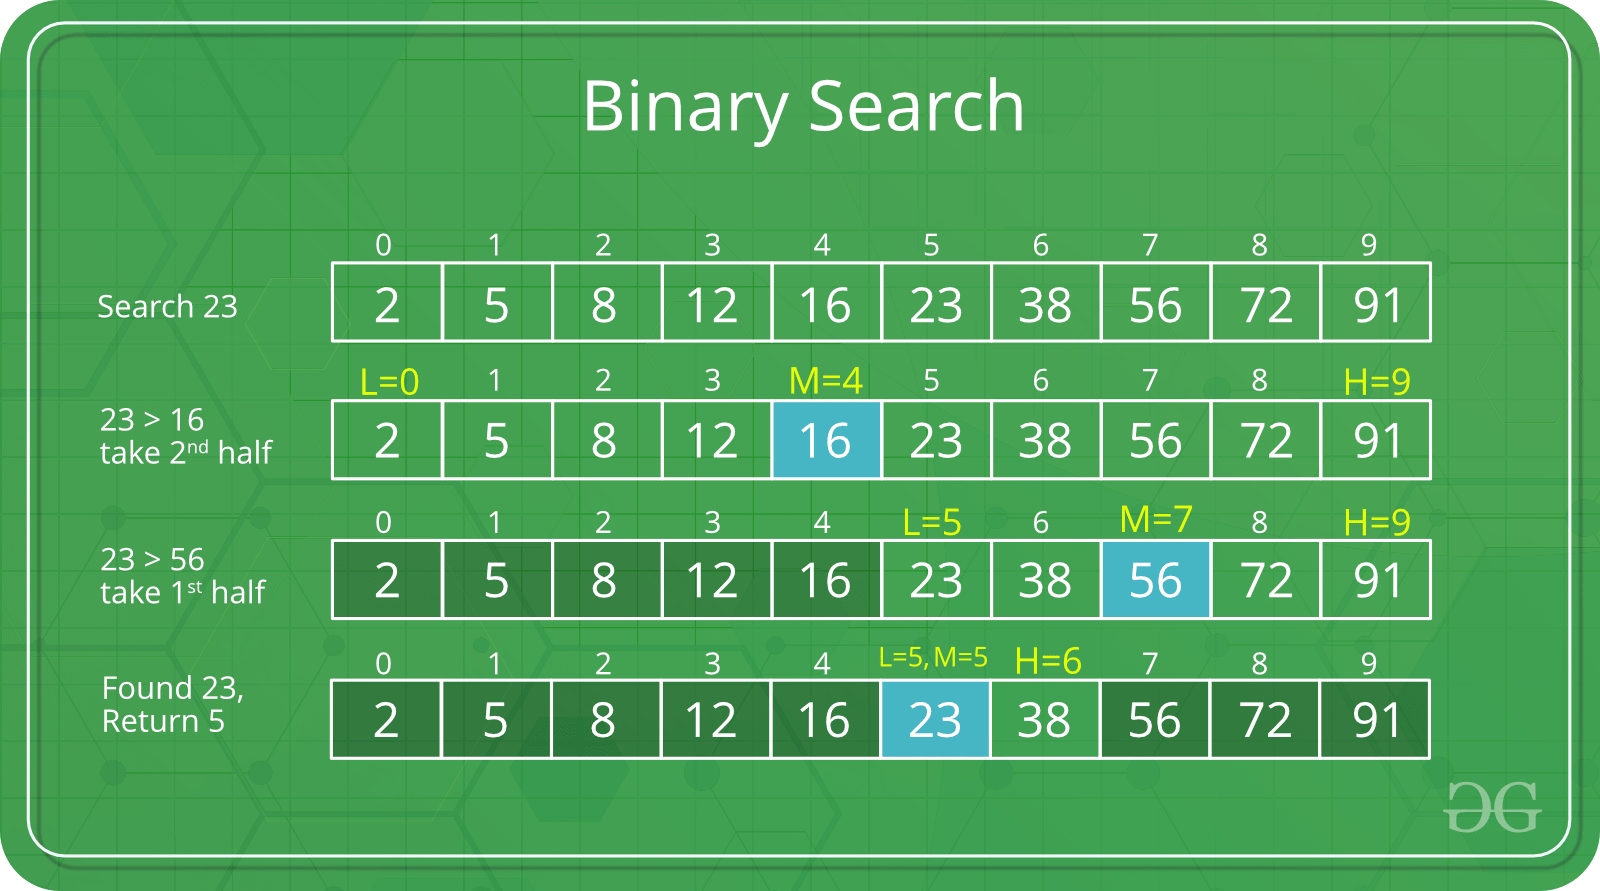
\includegraphics[width=.75\textwidth]{./img/binary-search.png}
  \end{figure}
\end{frame}

\begin{frame}[fragile]
  \scriptsize
  \begin{minted}[bgcolor=Black]{c}
int bsearch(int start, int end, int a[], int value){
  int mid = (start + end) / 2;

  if(a[mid] == value)
     return mid;
  else if(start >= end)
    return -1;
  else if(value > a[mid])
    return bsearch(mid + 1, end, a, value);
  else
    return bsearch(start, mid - 1 , a, value);
}
  \end{minted}
\end{frame}

\section{Multidimensional arrays}

\begin{frame}[fragile]
  \frametitle{Multidimensional Arrays}
  \begin{itemize}
    \item
      If element of an array is array itself, it will be Multidimensional array

    \begin{minted}[bgcolor=Black]{c}
int t[10][20];
    \end{minted}
    \item $10 \times 20$ matrix of integers
    \begin{minted}[bgcolor=Black]{c}
t[1][1];
// t[1,1] // compile error
    \end{minted}
    \item Integer variable in location (1,1)
  \end{itemize}
\end{frame}

\begin{frame}[fragile]
  \frametitle{Initializing Multidimensional Arrays}
  \begin{itemize}
    \begin{minted}[bgcolor=Black]{c}
int num[2][3] = {1, 2, 0, 3, 4, 7};
int num[2][3] = { {1, 2, 0}, {3, 4, 7} };
    \end{minted}
    \item num[0][2] is 0, num[1][0] is 3
    \begin{minted}[bgcolor=Black]{c}
int num[5][3] = { {1, 2, 0}, {3, 4, 7} };
    \end{minted}
    \item num[2][2] is 0, num[1][2] is 7
  \end{itemize}
\end{frame}

\begin{frame}[fragile]
  \begin{itemize}
    \begin{minted}[bgcolor=Black]{c}
int num[2][3][2] = { { {1, 2}, {3, 4}, {5, 6} }, { {1}, {2}, {3} } };
    \end{minted}
    \item num[0][2][1] is 6, num[1][0][1] is 0
    \begin{minted}[bgcolor=Black]{c}
int num[][2] = { {1, 1}, {2, 2}, {3, 3} };
    \end{minted}
    \item num[1][1] is 2, num[2][0] is 3
    \item
      All dimentions
      \textbf{\color{Orange} except the first one} \textbf{\color{Yellow} are required} in
      initiation
  \end{itemize}
\end{frame}

\begin{frame}[fragile]
  \frametitle{Multidimensional Arrays in Functions}
  \begin{itemize}
    \item
      Can be used as input of functions. All dimensions except the first one
      {\color{YellowOrange} must} be given.

    \begin{minted}[bgcolor=Black]{c}
void func(int a[10][20][5]);
    \end{minted}
    \begin{itemize}
      \item Input is a $10 \times 20 \times 5$ integer matrix
    \end{itemize}
    \begin{minted}[bgcolor=Black]{c}
void func(int a[][20][30], int size);
    \end{minted}
    \begin{minted}[bgcolor=Black]{c}
void func(int size1, int size2, int a[size1][size2]);
    \end{minted}
    \begin{itemize}
      \item
        Input is a matrix of integers that both rows and columns are variable

    \end{itemize}
  \end{itemize}
\end{frame}

\begin{frame}[fragile]
  \frametitle{Matrix Transpose}
  \begin{minted}[bgcolor=Black]{c}
#define SIZE 5

void swap(int a[SIZE][SIZE], int i, int j) {
  int tmp;
  tmp = a[i][j];
  a[i][j] = a[j][i];
  a[j][i] = tmp;
}

void transpose(int a[][SIZE]) {
  int i, j;
  for(i = 0; i < SIZE; i++)
    for(j = i; j < SIZE; j++)
      swap(a, i, j);
}
  \end{minted}
\end{frame}

\begin{frame}[fragile]
  \frametitle{Matrix Print}
  \begin{minted}[bgcolor=Black]{c}
#include <stdio.h>

void display_matrix(int n_rows, int n_cols, int matrix[n_rows][n_cols]) {
  int row, column;

  for (row = 0; row < n_rows; row++) {
    for (column = 0; column < n_cols; column++)
      printf("%5d ", matrix[row][column]);
    printf("\n");
  }
}

int main (void){
  int sample[3][5] =
    {
      { 7, 16, 55, 13, 12 },
      { 12, 10, 52, 0, 7 },
      { -2, 1, 2, 4, 9 }
    };
    printf("Original matrix:\n");
    display_matrix(3, 5, sample);
}
  \end{minted}
\end{frame}

\begin{frame}[fragile]
  \begin{minted}[bgcolor=Black]{output}
Original matrix:
    7    16    55    13    12
   12    10    52     0     7
   -2     1     2     4     9
  \end{minted}
\end{frame}

\begin{frame}
  \frametitle{Array In Memory}
  \begin{figure}
    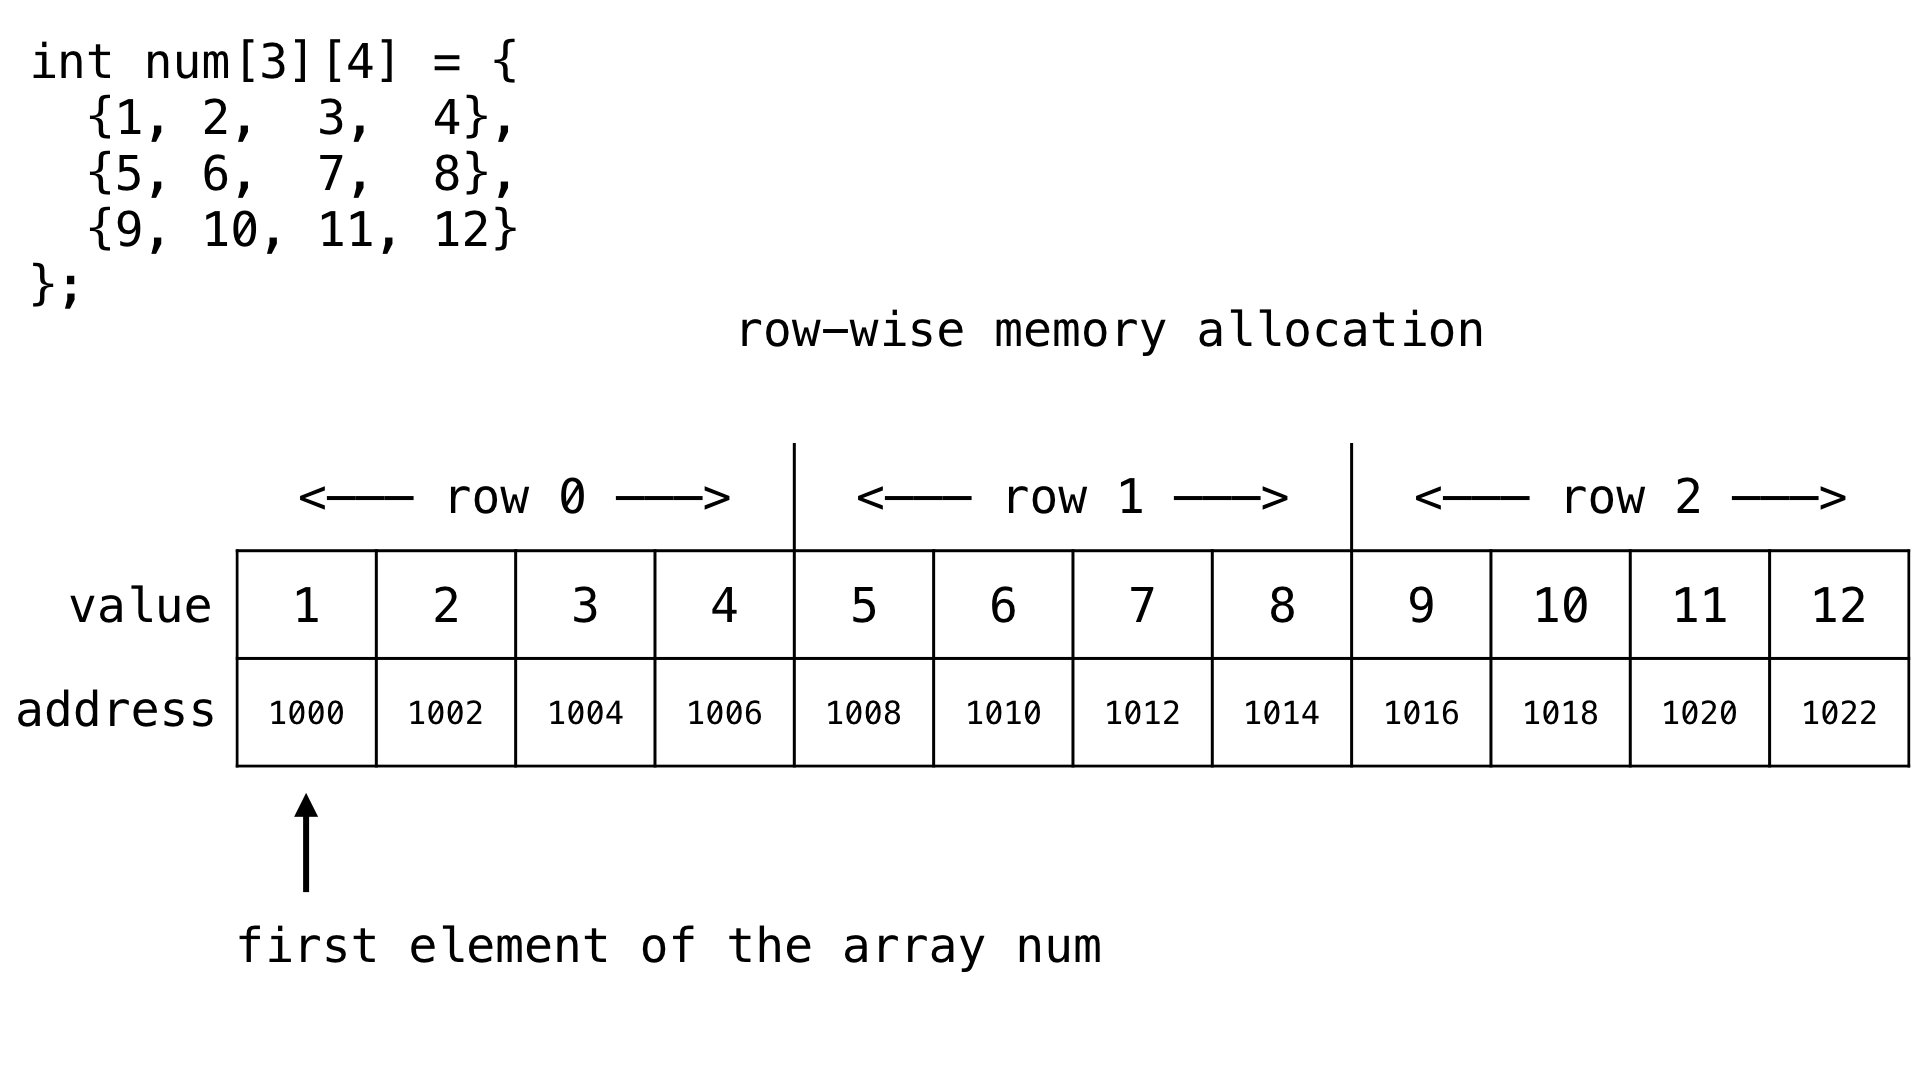
\includegraphics[width=.75\textwidth]{./img/arrays-in-memory.png}
  \end{figure}
\end{frame}

\begin{frame}[fragile]
  \begin{minted}[bgcolor=Black]{c}
#include <stdio.h>

int main() {
  int arr[][3] = { {1, 2, 3}, {4, 5, 6}, {7, 8, 9} };

  printf("%lu\n", sizeof(arr)); // 36 = 9 * 4 = 9 * sizeof(int)
}
  \end{minted}
  \begin{block}{}
    There is no way to findout dimensions of an array
  \end{block}
\end{frame}

\section{String}

\begin{frame}[fragile]
  \frametitle{Introduction}
  \begin{itemize}
    \item Until now
    \begin{itemize}
      \item We have seen strings in \textit{\color{Cyan} printf}
      \item Our old definition: string is a set of char between `` '' 😂
      \begin{minted}[bgcolor=Black]{c}
printf("This is a string\n");
printf("This is %s\n", "a string\n");
      \end{minted}
    \end{itemize}
    \item Strings:
    \begin{itemize}
      \item An array of chars
      \item Terminated by the \textit{\color{Orange} null char} \mintinline{c}|'\0'|
    \end{itemize}
  \end{itemize}
\end{frame}

\begin{frame}[fragile]
  \frametitle{Strings in C}
  \begin{itemize}
    \item Since strings are array
  \end{itemize}
  \begin{minted}[bgcolor=Black]{c}
char str1[] = {'p', 'r', 'o', 'g', 'r', 'a', 'm', '\0'};
char str2[8] = "program";
char str3[] = "program";
char *str4 = "program"; //we will see later
  \end{minted}
  \begin{table}
  \begin{tabular}{*{8}{c}}
    \toprule
    'p' &
    'r' &
    'o' &
    'g' &
    'r' &
    'a' &
    'm' &
    {\color{Orange} '\textbackslash 0'} \\
    \bottomrule
  \end{tabular}
  \end{table}
\end{frame}

\begin{frame}[fragile]
  \frametitle{Reading \& Writing Strings}
  \begin{itemize}
    \item \textit{\color{SpringGreen} printf} can be used to print strings
    \begin{minted}[bgcolor=Black]{c}
printf("program");
printf("%s", "program");
    \end{minted}
  \end{itemize}
  \begin{itemize}
    \item \textit{\color{LimeGreen} scanf} can be used to read strings
    \begin{minted}[bgcolor=Black]{c}
char str[200];
scanf("%s", str);
    \end{minted}
    \item Initial white spaces are ignored
    \item
      Read until \textit{\color{Orange} space} or
      \mintinline{c}|'\n'| (which is replaced by \mintinline{c}|\0|)

    \item We must allocate \textbf{\color{RubineRed} sufficient size}
  \end{itemize}
\end{frame}

\begin{frame}
  \frametitle{Reading \& Writing Strings (cont’d)}
  \begin{itemize}
    \item
      \textit{\color{YellowOrange} puts(str)} is \textsc{\color{Cyan} very} simple version of
      \textit{\color{LimeGreen}printf}

    \begin{itemize}
      \item Can only be used to print strings
      \item Adds \mintinline{c}|'\n'| to end of string
    \end{itemize}
    \item
      \textit{\color{YellowOrange} gets(char str[])} can be used to read
      strings

    \item
      \textit{\color{YellowOrange} gets} does
      \textsc{\color{RubineRed} not} ignore the white spaces

    \begin{itemize}
      \item Read until \mintinline{c}|'\n'|
    \end{itemize}
    \item String should be large enough
  \end{itemize}
\end{frame}

\section{String functions}

\begin{frame}[fragile]
  \frametitle{String Library}
  \begin{itemize}
    \item Access to string library by
    \begin{minted}[bgcolor=Black]{c}
#include <string.h>
    \end{minted}
    \item Many functions to work with strings
    \begin{itemize}
      \item Find the length of string
      \item Compare strings
      \item Copy strings
      \item Search in strings
      \item \ldots
    \end{itemize}
  \end{itemize}
\end{frame}

\begin{frame}[fragile]
  \frametitle{Length of String}
  \begin{itemize}
    \item <span class="hl-orange">strlen(str)</span>: Length of string
    \item
      From start to first occurrence of the
      \textsc{\color{LimeGreen} null} char

  \end{itemize}
  \begin{minted}[bgcolor=Black]{c}
char str[] = "This is test";
char str1[10] = {'a', 'b', '\0', 'c', '\0'};
strlen(str)  // returns 12
strlen(str1) // returns 2 😱
  \end{minted}
\end{frame}

\begin{frame}
  \frametitle{Compare Strings}
  \begin{itemize}
    \item str1 and str2 are compared as follows
    \begin{itemize}
      \item
        Compare \textit{\color{LimeGreen} char by char} from
        \textit{\color{Cyan} left to right} until str1 and str2 has same
        chars.

      \item In the first different char
      \begin{itemize}
        \item if (char of str1 < char of str2) \textrightarrow str1 < str2
      \end{itemize}
      \item if (both string finish) \textrightarrow str1 = str2
    \end{itemize}
    \item
      <span class="hl-orange">strcmp(str1, str2)</span>:compare str1 and str2
  \end{itemize}
\end{frame}

\begin{frame}[fragile]
  \frametitle{Compare Strings: Examples}
  \begin{minted}[bgcolor=Black]{c}
char s1[] = "abc";
char s2[] = "abc";
i = strcmp(s1, s2); // i = 0, s1 is equal to s2

char s3[] = "abc";
char s4[] = "abx";
i = strcmp(s3, s4); // i = -1, s3 is lower than s4

char s5[] = "axc";
char s6[] = "abc";
i = strcmp(s5, s6); // i = 1, s5 is greater than s6

char s7[] = "ab";
char s8[] = "abc";
i = strcmp(s7, s8); // i = -1, s7 is lower than s8

char s9[] = "abc";
char s10[] = "aBc";
i = strcmp(s9, s10); // i = 1, s9 is greater than s10
  \end{minted}
\end{frame}

\begin{frame}[fragile]
  \frametitle{Compare Strings}
  \begin{itemize}
    \item <span class="hl-orange">strcmpi(str1, str2)</span>
    \item Compares str1 and str2 similar to strcmp
    \item But ignores uppercase/lowercase difference
  \end{itemize}
  \begin{minted}[bgcolor=Black]{c}
char str1[] = "ABC";
char str2[] = "abC";
strcmpi(str1, str2) // 0
  \end{minted}
\end{frame}

\begin{frame}
  \frametitle{Copy Strings}
  \begin{itemize}
    \item Strings should be copied char by char
    \item
      \mintinline{c}|strcpy(dst_str, src_str)|: copy the
      \mintinline{c}|src_str| to the
      \mintinline{c}|dst_str| including NULL

    \item
      \mintinline{c}|src_str| is a
      \textbf{\color{YellowOrange} constant} string

    \item
      \mintinline{c}|dst_str| should have
      \textbf{\color{YellowOrange} sufficient size}
  \end{itemize}
\end{frame}

\begin{frame}[fragile]
  \frametitle{Copy Strings: Example}
  \begin{minted}[bgcolor=Black]{c}
char str1[] = "Test String";
char str2[20];

strcpy(str2, str1);

printf("%s\n", str2); // Test String
printf("%s\n", str1); // Test String
  \end{minted}
\end{frame}

\begin{frame}
  \frametitle{Concatenate Strings}
  \begin{itemize}
    \item
      \mintinline{c}|strcat(dst_str, src_str)|: Append the
      \mintinline{c}|src| string to the end of
      \mintinline{c}|dst| including NULL
    \item
      \mintinline{c}|src| is a
      \textbf{\color{YellowOrange} constant} string
    \item
      \mintinline{c}|dst| should have
      \textbf{\color{YellowOrange} sufficient space}
  \end{itemize}
\end{frame}

\begin{frame}[fragile]
  \frametitle{Concatenate Strings: Example}
  \begin{minted}[bgcolor=Black]{c}
char str1[] = "String";
char str2[20] = "Test ";

strcat(str2, str1);

printf("%s\n", str2); // Test String
  \end{minted}
\end{frame}

\begin{frame}
  \frametitle{Sized Version of the Functions}
  \begin{itemize}
    \item \textit{\color{YellowOrange} strncpy(dst, src, n):}
    \begin{itemize}
      \item
        copys \textit{\color{RubineRed} n} chars from
        \textit{\color{Cyan} src} to \textit{\color{Melon} dst}

      \item if(strlen(src) > n)
      \begin{itemize}
        \item Copies n chars to \textit{\color{Melon} dst}
        \item
          Does not add \mintinline{c}|'\0'| to end of \textit{\color{Melon} dst}

      \end{itemize}
      \item if(strlen(src) < n)
      \begin{itemize}
        \item
          Copy \textit{\color{Cyan} src} to
          \textit{\color{Melon} dst}

        \item
          Add n – strlen(src) – 1 \mintinline{c}|'\0'|s to end of
          dst

        \item \textit{\color{Melon} dst} must be large enough
        \item n < size of dst
      \end{itemize}
    \end{itemize}
  \end{itemize}
\end{frame}

\begin{frame}
  \frametitle{Sized Version of the Functions}
  \begin{itemize}
    \item <span class="hl-orange">strncmp(str1, str2, n):</span>
    \begin{itemize}
      \item compares the first <span class="hl-green">x</span> chars
      \item
        <span class="hl-green">x</span> = min( n, strlen(str1) + 1,
        strlen(str2) + 1 )

    \end{itemize}
    \item \mintinline{c}|strncat(dst, src, n)|:
    \begin{itemize}
      \item
        Appends the <span class="hl-green">x</span> chars from src to dst

      \item \textit{\color{RubineRed} x} = min{ n, strlen(src) }
      \item
        Adds \mintinline{c}|'\0'| to end of dst \textbf{\color{RubineRed} unlike}
        \textit{\color{Cyan} strncpy}

      \item dst must be large enough
    \end{itemize}
  \end{itemize}
\end{frame}

\begin{frame}[fragile]
  \begin{minted}[bgcolor=Black]{c}
char s1[] = "Hello";
char s2[] = "Hell";

printf("%d\n", strcmp(s1, s2));     // s1 > s2
printf("%d\n", strncmp(s1, s2, 2)); // s1 == s2
printf("%d\n", strncmp(s1, s2, 4)); // s1 == s2
printf("%d\n", strncmp(s1, s2, 5)); // s1 > s2
  \end{minted}
\end{frame}

\begin{frame}[fragile]
  \frametitle{Numbers and Strings: number \textrightarrow string}
  \begin{itemize}
    \item To convert a number to string
    \begin{minted}[bgcolor=Black]{c}
#include <stdio.h> // sprintf

char str1[100];

int i = 100;
sprintf(str1, "%d", i); // str1 = “100”

float f = 10.11;
sprintf(str1, "%0.2f", f); // str1 = “10.11”

    \end{minted}
    \item
      String <span class="hl-orange">str1</span> should have
      <span class="hl-material">sufficient size</span>

  \end{itemize}
\end{frame}

\begin{frame}[fragile]
  \frametitle{Numbers and Strings: string \textrightarrow number}
  \begin{itemize}
    \item To convert from strings to numbers
    \begin{minted}[bgcolor=Black]{c}
#include <stdlib.h> // atoi, atof
#include <stdio.h> // sscanf

char str1[] = "10";
int i;
i = atoi(str1); // i = 10
sscanf(str1, "%d", &i); // i = 10

char str2[] = "20.44";
double f;
f = atof(str2); // f = 20.44
sscanf(str2, "%lf", &f); // f = 20.44
    \end{minted}
  \end{itemize}
\end{frame}

\begin{frame}[fragile]
  \frametitle{String as Array}
  \begin{itemize}
    \item Strings are array of chars
    \item We work on arrays element by element
    \item We can work on strings char by char
    \begin{minted}[bgcolor=Black]{c}
char str1[] = "100000";
str1[2] = '2';
    \end{minted}
    \item We can pass strings to functions
  \end{itemize}
\end{frame}

\begin{frame}[fragile]
  \frametitle{Array of Strings}
  \begin{itemize}
    \item 2 dimensional array, each row is a string
    \begin{minted}[bgcolor=Black]{c}
char numeri[][8] = { "zero", "uno", "due", "tre", "quattro" }; 🇮🇹
char numeri[][] = { "zero", "uno", "due", "tre", "quattro" }; // Compile Error
    \end{minted}
    \begin{table}
    \begin{tabular}{*{8}{c}}
      \toprule
        'z' &
        'e' &
        'r' &
        'o' &
        '\textbackslash 0' &
        '\textbackslash 0' &
        '\textbackslash 0' &
        '\textbackslash 0' \\
      \midrule
        'u' &
        'n' &
        'o' &
        '\textbackslash 0' &
        '\textbackslash 0' &
        '\textbackslash 0' &
        '\textbackslash 0' &
        '\textbackslash 0' \\
      \midrule
        'd' &
        'u' &
        'e' &
        '\textbackslash 0' &
        '\textbackslash 0' &
        '\textbackslash 0' &
        '\textbackslash 0' &
        '\textbackslash 0' \\
      \midrule
        't' &
        'r' &
        'e' &
        '\textbackslash 0' &
        '\textbackslash 0' &
        '\textbackslash 0' &
        '\textbackslash 0' &
        '\textbackslash 0' \\
      \midrule
        'q' &
        'u' &
        'a' &
        't' &
        't' &
        'r' &
        'o' &
        '\textbackslash 0' \\
      \bottomrule
    \end{tabular}
    \end{table}
  \end{itemize}
\end{frame}

\begin{frame}
  \frametitle{ctype.h}
  \begin{itemize}
    \item Many function to work on chars
    \begin{itemize}
      \item Check digit
      \item Check alphabetic
      \item Check lower or upper case
      \item Convert from/to upper/lower case
    \end{itemize}
  \end{itemize}
\end{frame}

\begin{frame}
  \frametitle{ctype.h}
  \begin{itemize}
    \item int isdigit(ch)
    \begin{itemize}
      \item Check ch is digital char or not
    \end{itemize}

    \pause

    \item int isalpha(ch)
    \begin{itemize}
      \item Check ch is alphabetic or not
    \end{itemize}

    \pause

    \item int islower(ch)
    \begin{itemize}
      \item Check ch is lowercase alphabetic or not
    \end{itemize}

    \pause

    \item int isupper(ch)
    \begin{itemize}
      \item Check ch is uppercase alphabetic or not
    \end{itemize}

    \pause

    \item char tolower(ch)
    \begin{itemize}
      \item Convert ch to lowercase and return it
    \end{itemize}

    \pause

    \item char toupper(ch)
    \begin{itemize}
      \item Convert ch to upper case and return it
    \end{itemize}
  \end{itemize}
\end{frame}

\section{Bugs and avoiding them}

\begin{frame}
  \frametitle{Common Bugs \& Avoiding them}
  \begin{itemize}
    \item Strings which are used as destination
    \begin{itemize}
      \item scanf, sprintf, strcpy, \ldots
      \item Must be large enough
    \end{itemize}
    \item Take care about the \mintinline{c}|'\0'|
    \begin{itemize}
      \item You should never destroy it, some library functions do!
    \end{itemize}
    \item
      Out of range array index!!!! (read/write, wrong size in function,
      multidimensional array memory)
  \end{itemize}
\end{frame}

\begin{frame}[fragile]
  \frametitle{Common Bugs \& Avoiding them}
  \begin{itemize}
    \item You cannot assign a value to array
    \scriptsize
    \begin{minted}[bgcolor=Black]{c}
int a[4], b[4];
a = b; // error: assignment to expression with array type
a = 4; // error: assignment to expression with array type
    \end{minted}
    \normalsize
    \item To debug
    \begin{itemize}
      \item Print the array index and corresponding value
    \end{itemize}
  \end{itemize}
\end{frame}

\end{document}
